\chapter{The old algorithm}

% Explain what the old algorithm does
% Explain what has changed


% The new algorithm is based on 

% \section{Definitions}



% TODO from meeting with Aarne
% Rename chapter to old algorithm make new chapter for new algorithm
% The kind of algorithm Forward something,  parsing
% One UD tree can be many GF trees

% Example of UD corresponding to several GF trees:
% grande famille francaice

% coffee or tea and soup
% not ambigous in UD, but the phrase is ambigous

% Can linearize wrong

% Church encoding of pairs

% Link to github

% Exempel före definition

% Synkategorimatiska ord behöver särskild syntax för att dom inte har någon egen kategori
% kategorimatiska ord är lexikal funktion (utan argument)
% synkategorimatiska ord kommer från linjariseringsregler för funktioner tar argument

% diskontinueliga saker, e.g. V2 med prepositioner är syncat
% multiword expressions är en nod i GF men olika i UD

% konjunktioner: första ordet är förälder medan alla andra ord har komma eller konjunktion som barn

% Intressant idé: Definiera en mappning mellan två GF-grammatiker

% Redundans: koppling åt båda håll för syncats

% Old version of gf2ud still exists in gf-shell

% Half time report

% Describe the annotation
% #fun
% #cat
% #auxfun - macros
% #auxcat

% Syncat: #morpho, #lemma, #word
% Used both directions

% Parameters aren't automatically handled, but you need to create auxfuns


% Auxfun are not type checked 

% Needed for halftime report:
% Write what the empty chapters will contain

\todo[inline]{Signposting: In this section we will explain ...}

In this chapter we first explain the annotations that are used to describe the mapping between gf trees and ud trees, then we will give a high level overview of the algorithm followed by going through a concrete example of how the algorithm works. Finally we will discuss some limitations of the old algorithms, which we will cover solutions of in the next chapter.

\section{Overview}

The whole process goes like this: first we do X (section XXX, then we do Y (section YYY)

Gf trees consist of functions and categories, UD trees consist of PoS annotations and dependency labels (plus some extra annotation)

\section{How annotations work}

In order for the program to know which UD Part of Speech (POS) corresponds to which GF Categories and how the GF functions relates to the UD dependency labels, we need to supply annotations which describe these correspondences. Most of these annotations are bidirectional and are used both by ud2gf and gf2ud.

First we have the \lstinline{#cat} annotation, which describes the mapping from GF categories and UD Part of Speech labels:

\begin{lstlisting}
    #cat GFCategory UD_POS
    #cat N NOUN
\end{lstlisting}

Secondly we have the \lstinline{#fun} annotation, which describes GF functions and which UD dependency label each argument of the function should have (see \autoref{fig:DetCN} for graphical representation of such an annotation). The type signature of the GF function is also required. Each function needs to have at least one head with the label \lstinline{head} and any number of children which are labeled with their corresponding UD dependency labels. It is also possible to add other UD annotations in brackets to a label.

\todo[inline]{How to give this listing a number and a label}
\begin{lstlisting}
    #fun GFFunctionName : FirstArgumentCat -> SecondArgumentCat -> ReturnCat ; first_ud_label second_ud_label
    #fun UseN : N -> CN ; head
    #fun DetCN  : Det -> CN -> NP ; det  head
\end{lstlisting}

The function \lstinline{UseN} only has a single argument (of type \lstinline{N}), so that is required to be the head, while the function \verb|DetCN| has two arguments, of types \verb|Det| and \verb|CN|, the first of which has the dependency label \verb|det|, while the second is the head. An illustration of this can be seen in \autoref{fig:DetCN}.

\begin{figure}
    \centering
    \begin{dependency}
        \begin{deptext}[column sep=0.4cm]
              % the \& cat \\
            % {\tt Det}\&{\tt CN}\&{\tt NP}\\
            {\tt Det}\&{\tt CN}\\
        \end{deptext}
        \depedge{2}{1}{det}
        \deproot{2}{head}
        % \wordgroup{1}{1}{2}{args}
        % \wordgroup{1}{3}{3}{res}
        % \groupedge[edge below]{args}{res}{\texttt{DetCN}}{2ex}
        \node (arg1) [below of = \wordref{1}{1}, yshift = -1ex]  {\texttt{Det}};
        \node (arg2) [below of = \wordref{1}{2}, yshift = -1ex]  {\texttt{CN}};
        \node (result) [right of = arg2, xshift = 1ex]  {\texttt{NP}};
        \node (function) [left of = arg1, xshift = -1.5ex]  {\texttt{DetCN :}};
          % Det} -> \subnode{arg2}{CN} -> NP}};
        \draw [->, thick] (arg1) -- (arg2);
        \draw [->, thick] (arg2) -- (result);
        \draw [->, very thick, dashed, gray] (arg1) -- (\wordref{1}{1});
        \draw [->, very thick, dashed, gray] (arg2) -- (\wordref{1}{2});
    \end{dependency} \\
    \caption{The UD shape that the function \texttt{DetCN} matches against.}
    \label{fig:DetCN}
\end{figure}

Both of these annotations are bidirectional and language-independent, since they only refer to the abstract syntax in GF.

%% TODO: Other 

% The different kinds of annotations in labels files
% Funs


%\section{Examples}

% When converting the sentence ``The cat is black'', from UD format to a GF format using ud2gf something happens
% 
% \begin{lstlisting}
% # gf, (gf2ud) original GF tree:
% UseCl TSim PPos (PredVP (DetCN the_Det (UseN cat_N)) (UseAP (PositA black_A)))
% # an3, (gf2ud) final annotated tree with nonlocal operations:
% @4: black black ADJ _  black_A A root
%     @2: cat cat NOUN Number=Sing  cat_N N nsubj
%         @1: the the DET _  the_Det Det det
%     @3: is be AUX Mood=Ind|Number=Sing|Person=3|Tense=Pres|VerbForm=Fin  UseAP VP cop
% 
% # ut, tree-structured UD tree:
% 4       black   black   ADJ     A       _       0       root    _       FUN=black_A
%     2   cat     cat     NOUN    N       Number=Sing     4       nsubj   _       FUN=cat_N
%         1       the     the     DET     Det     _       2       det     _       FUN=the_Det
%     3   is      be      AUX     VP      Mood=Ind|Number=Sing|Person=3|Tense=Pres|VerbForm=Fin   4       cop     _       FUN=UseAP
% 
% # ud, UD tree in CoNLLU format:
% # sent_id = gfud1000001
% # text = the cat is black
% 1       the     the     DET     Det     _       2       det     _       FUN=the_Det
% 2       cat     cat     NOUN    N       Number=Sing     4       nsubj   _       FUN=cat_N
% 3       is      be      AUX     VP      Mood=Ind|Number=Sing|Person=3|Tense=Pres|VerbForm=Fin   4       cop     _       FUN=UseAP
% 4       black   black   ADJ     A       _       0       root    _       FUN=black_A
% 
% \end{lstlisting}

\section{Overview of algorithm}

We start with a UD tree (e.g. \autoref{fig:the_black_cat_ud}), then we first map each Part Of Speech label into a GF category and then assign lexical entries to each node in the tree according to those categories. For example, the string ``cat'', with POS ``NOUN'' would become \lstinline|cat_N : N|, which is a nullary GF function of type/category \lstinline|N|. This is done through GF's built parse function. In some cases, there are multiple possible GF expressions of the correct type and linearization, in these cases all of the possibilities are added.

Now we have a ud tree with a list of gf trees at each node (\autoref{fig:the_black_cat_ud_gf}). We start traversing the tree, depth first, when we reach a leaf, we start processing it

The main loop is: go through all the available functions and apply as many as possible and add the result to our list

When no more functions can be applied, we go to the next node in the tree.

\subsection{Example: The black cat}

For a very simple initial example, we start with the noun-phrase ``the black cat'', which has the following UD representation:

\begin{figure}[H]
    \centering
    %% the black cat
    \setlength{\unitlength}{0.2mm}
    % \begin{picture}(158.0,90.0)
    %   \put(0.0,0.0){the}
    %   \put(37.0,0.0){black}
    %   \put(92.0,0.0){cat}
    %   \put(0.0,15.0){{\tiny DET}}
    %   \put(37.0,15.0){{\tiny ADJ}}
    %   \put(92.0,15.0){{\tiny NOUN}}
    %   \put(56.0,30.0){\oval(88.73913043478261,66.66666666666667)[t]}
    %   \put(11.630434782608695,35.0){\vector(0,-1){5.0}}
    %   \put(41.0,66.33333333333334){{\tiny det}}
    %   \put(74.5,30.0){\oval(49.54545454545455,33.333333333333336)[t]}
    %   \put(49.72727272727273,35.0){\vector(0,-1){5.0}}
    %   \put(59.5,49.66666666666667){{\tiny amod}}
    %   \put(107.0,90.0){\vector(0,-1){60.0}}
    %   \put(112.0,80.0){{\tiny root}}
    % \end{picture}
    \begin{dependency}
        \begin{deptext}[column sep=0.4cm]
              the \& black \& cat \\
            {\tt DET}\&{\tt ADJ}\&{\tt NOUN}\\
        \end{deptext}
        \depedge{3}{1}{det}
        \depedge{3}{2}{amod}
        \deproot{3}{root}
    \end{dependency} \\
    \caption{``The black cat'' as a UD tree}
    \label{fig:the_black_cat_ud}
\end{figure}

And we use the following GF abstract syntax:

\todo[inline]{Place these side-by-side}
\begin{verbatim}
  cat
    Det CN NP AP N A;
  fun
    -- Syntactic functions
    DetCN  : Det -> CN -> NP;
    ModCN  : AP  -> CN -> CN;
    UseN   : N         -> CN;
    PositA : A         -> AP;

    -- Lexical functions:
    the_Det : Det;
    black_A : A;
    cat_N : N;
\end{verbatim}
and the following corresponding dependency configuration (labels-file):
\begin{verbatim}
    #fun DetCN  : Det -> CN -> NP ; det  head
    #fun ModCN  : AP  -> CN -> CN ; amod head
    #fun UseN   : N         -> CN ; head
    #fun PositA : A         -> AP ; head
    
    #cat A                        ; ADJ
    #cat Det                      ; DET
    #cat N                        ; NOUN
\end{verbatim}

Notice how only the lexical categories (returned by lexical functions) have a corresponding UD Part of Speech. This is a distinction between GF's phrase structure structure grammar, which uses phrasal categories covering entire phrases, and UD's dependency grammar, where the individual words are annotated with a Part of Speech. \todo{Write a section in the introduction to refer back to here.}

The first step is to parse each word in the UD tree into their corresponding lexical GF functions. We use the configuration in the labels-file to convert UD-part-of-speech into their corresponding GF categories.
\begin{verbatim}
    DET -> Det
    ADJ -> A
    NOUN -> N
\end{verbatim}
And then we use the GF parser on each individual lemma (word in the dictionary form), with the category we just got\todo{Explain that gf parser wants to know which category to parse in}.
This gives the tree in \autoref{fig:the_black_cat_ud_gf}. Notice how the words have been replaced by GF lexical functions and the POS annotations have been replaced by GF Categories. The UD dependency labels still remain.

% TODO: Fix this so it's not so ugly
\begin{figure}[H]
    \centering
    % %% the black cat
    % \setlength{\unitlength}{0.2mm}
    % \begin{picture}(158.0,90.0)
    %   \put(-30.0,0.0){the$_{Det}$}
    %   \put(27.0,0.0){black$_A$}
    %   \put(92.0,0.0){cat$_N$}
    %   \put(0.0,15.0){{\tiny Det}}
    %   \put(37.0,15.0){{\tiny A}}
    %   \put(92.0,15.0){{\tiny N}}
    %   \put(56.0,30.0){\oval(88.73913043478261,66.66666666666667)[t]}
    %   \put(11.630434782608695,35.0){\vector(0,-1){5.0}}
    %   \put(41.0,66.33333333333334){{\tiny det}}
    %   \put(74.5,30.0){\oval(49.54545454545455,33.333333333333336)[t]}
    %   \put(49.72727272727273,35.0){\vector(0,-1){5.0}}
    %   \put(59.5,49.66666666666667){{\tiny amod}}
    %   \put(107.0,90.0){\vector(0,-1){60.0}}
    %   \put(112.0,80.0){{\tiny root}}
    % \end{picture}
    \begin{dependency}
        \begin{deptext}[column sep=0.4cm]
              {\tt the\_Det}\&{\tt black\_A}\&{\tt cat\_N}\\
            {\tt Det}\&{\tt A}\&{\tt N}\\
        \end{deptext}
        \depedge{3}{1}{det}
        \depedge{3}{2}{amod}
        \deproot{3}{root}
    \end{dependency} \\
    \caption{``The black cat'' as a UD tree, with GF lexicon entries inserted}
    \label{fig:the_black_cat_ud_gf}
\end{figure}

%% I was here

% In the case of ``the black cat sees us today'', we go down the tree until we reach ``the'', and nothing can be done there, so we continue

After converting UD POS annotations to GF categories and parsing words to GF lexical functions, we start traversing the UD tree. The tree is processed from the bottom up, starting with the leaves. Since \lstinline{cat_N} has unprocessed children we keep going down and reach \lstinline{the_Det}. We look through the list of available functions and see that the only function that takes a \lstinline{Det} as an argument takes several arguments, so it can't be applied to a leaf node like this. There is nothing to be done here, so we continue.


\begin{figure}[H]
    \centering
    \subcaptionbox{``black'' as an adjective : A}[0.4\textwidth]
        {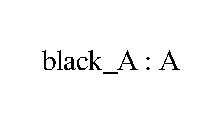
\includegraphics[scale=0.75]{thesis/figure/black_cats/black_A_gf.eps}}
    \caption{The available GF trees on the word ``black'' before the first iteration}\label{fig:black iter 0}
\end{figure}

Next we get to ``black'', with the available tree \lstinline|black_A| (\autoref{fig:black iter 0}) and here we can apply \lstinline|PositA : A -> AP ; head|, which converts an adjective into an Adjectival Phrase (AP), so now the available trees on ``black'' are
\lstinline|[black_A : A, PositA black_A : AP]| (\autoref{fig:black iter 0}), no more functions can be applied here, so we continue.

\begin{figure}[H]
    \centering
    \subcaptionbox{``black'' as an adjective : A}[0.4\textwidth]
        {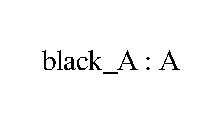
\includegraphics[scale=0.75]{thesis/figure/black_cats/black_A_gf.eps}}
    \subcaptionbox{``black'' as an adjectival phrase: AP}[0.4\textwidth]
        {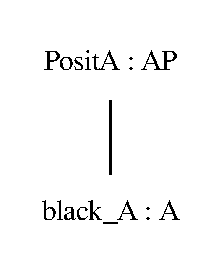
\includegraphics[scale=0.75]{thesis/figure/black_cats/black_AP_gf.eps}}
    \caption{The available GF trees on the word ``black'' after the first iteration}\label{fig:black iter 1}
\end{figure}

% A picture like 3.2, but with both the subtrees above attached to the word "black_A"

Now we are done with all the children of ``cat'', so we can start processing it. We have \lstinline|cat_N : N|. 

\begin{figure}[H]
    \centering
    \subcaptionbox{``cat'' : N}
        {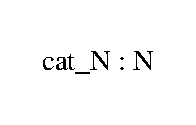
\includegraphics[scale=0.75]{thesis/figure/black_cats/cat_N_gf.eps}}
    \caption{The available GF trees on the word ``cat'' before the first iteration}\label{fig:cat iter 0}
\end{figure}

Looking through all the functions, only \lstinline|UseN : N -> CN ; head| takes an N as an argument, so that's the one that's applied, giving us \lstinline|UseN cat_N : CN|. Now we have the trees in \autoref{fig:cat iter 1}
% \begin{lstlisting}
%     cat_N : N
%     UseN cat_N : CN
% \end{lstlisting}

\begin{figure}[H]
    \centering
    \subcaptionbox{``cat'' as a noun : N}[0.4\textwidth]
        {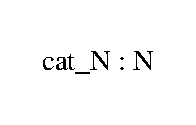
\includegraphics[scale=0.75]{thesis/figure/black_cats/cat_N_gf.eps}}
    \subcaptionbox{``cat'' as a common noun: CN}[0.4\textwidth]
        {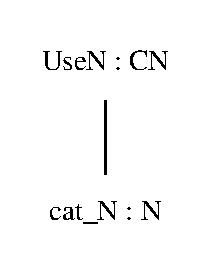
\includegraphics[scale=0.75]{thesis/figure/black_cats/cat_CN_gf.eps}}
    \caption{The available GF trees on the word ``cat'' after the first iteration}\label{fig:cat iter 1}
\end{figure}

In the next iteration we have a \lstinline|CN| available and can apply either of the functions
\begin{lstlisting}
    DetCN : Det -> CN -> NP ; det head
    ModCN : AP -> CN -> CN  ; amod head
\end{lstlisting}
Let us verify that these are possible to apply: For \lstinline|DetCN| we need a tree of type $Det$ with the $det$ ud label for the relation and indeed, the word ``the'' has the $det$ label on the relation to ``cat'' and we have the tree \lstinline|the_Det : Det| available on ``the''. Secondly we need a $CN$ at the head and since our current head is ``cat'' and we have \lstinline|UseN cat_N : CN|, that fits perfectly giving us \lstinline|DetCN the_Det (UseN cat_N) : NP|. With similar reasoning for \lstinline{ModCN}, we have ``black'' with UD-label $amod$ and one of the available trees for ``black'' is \lstinline|PositA black_A : AP| which has the correct category, which allows us to construct \lstinline|ModCN (PositA black_A) (UseN cat_N) : CN|. After this we have the trees in \autoref{fig:cat iter 2}

\begin{figure}[H]
    \centering
    \subcaptionbox{cat : N\label{cat_N}}
        {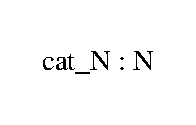
\includegraphics[scale=0.75]{thesis/figure/black_cats/cat_N_gf.eps}}
    \subcaptionbox{cat : CN\label{cat_CN}}
        {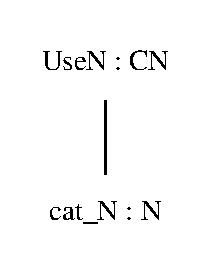
\includegraphics[scale=0.75]{thesis/figure/black_cats/cat_CN_gf.eps}}
    \subcaptionbox{the cat : NP\label{the_cat_NP}}
        {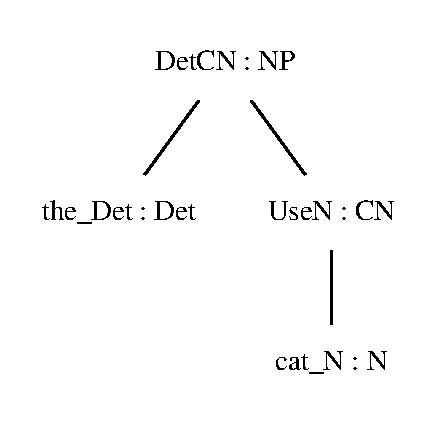
\includegraphics[scale=0.75]{thesis/figure/black_cats/the_cat_NP_gf.eps}}
    \subcaptionbox{black cat : CN\label{black_cat_CN}}
        {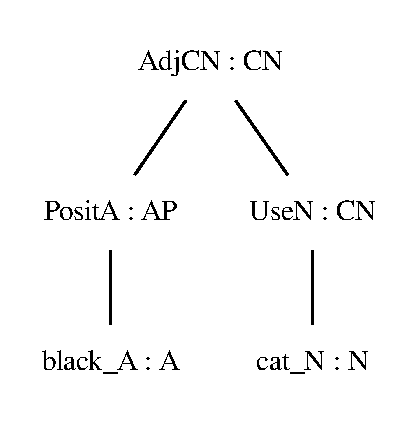
\includegraphics[scale=0.75]{thesis/figure/black_cats/black_cat_CN_gf.eps}}
    \caption{The four available trees on the word ``cat'' after the second iteration}\label{fig:cat iter 2}
\end{figure}

After this iteration we have two trees on ``cat'' which both have the same category $CN$, namely
\begin{lstlisting}
    UseN cat_N : CN
    ModCN (PositA black_A) (UseN cat_N) : CN
\end{lstlisting}
and one of them is a strict superset of the other when it comes to words covered, the first only covers ``cat'' while the second covers both ``black'' and ``cat''. This means we can prune the redundant tree \lstinline{UseN cat_N}.

\begin{figure}[H]
    \centering
    \subcaptionbox{Cat\label{ci2p:cat_N}}
        {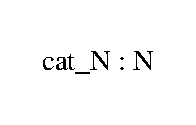
\includegraphics[scale=0.75]{thesis/figure/black_cats/cat_N_gf.eps}}
    \subcaptionbox{The cat\label{ci2p:the_cat_NP}}
        {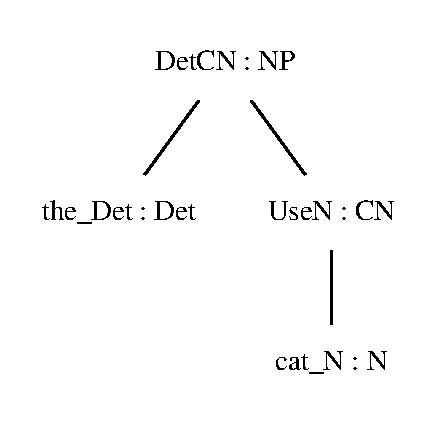
\includegraphics[scale=0.75]{thesis/figure/black_cats/the_cat_NP_gf.eps}}
    \subcaptionbox{Black cat\label{ci2p:black_cat_CN}}
        {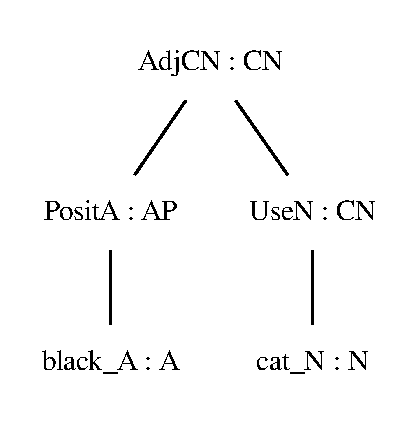
\includegraphics[scale=0.75]{thesis/figure/black_cats/black_cat_CN_gf.eps}}
    \caption{The three available trees on the word ``cat'' after the second iteration after pruning. Tree (b) will not be a subtree of the final tree}\label{fig:cat iter 2 pruned}
\end{figure}

After this pruning, the available trees on the ``cat'' node are (\autoref{fig:cat iter 2 pruned})
\begin{lstlisting}
    cat_N : N
    DetCN the_Det (UseN cat_N) : NP
    ModCN (PositA black_A) (UseN cat_N) : CN
\end{lstlisting}
After this step, one function is still possible to apply, namely $DetCN$, which can be applied to our new $CN$ together with \lstinline{the_Det} like before, giving us the new tree
\begin{lstlisting}
    DetCN the_Det (ModCN (PositA black_A) (UseN cat_N)) : NP
\end{lstlisting}

\begin{figure}[H]
    \centering
    \subcaptionbox{Cat : N\label{ci3:cat_N}}
        {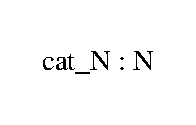
\includegraphics[scale=0.75]{thesis/figure/black_cats/cat_N_gf.eps}}
    \subcaptionbox{The cat : NP\label{ci3:the_cat_NP}}
        {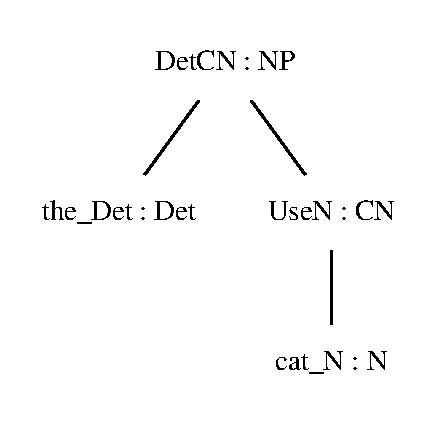
\includegraphics[scale=0.75]{thesis/figure/black_cats/the_cat_NP_gf.eps}}
    \subcaptionbox{Black cat : CN\label{ci3:black_cat_CN}}
        {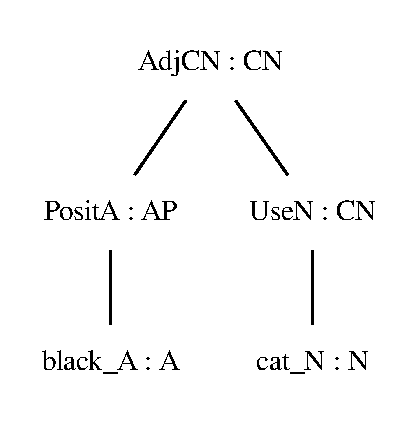
\includegraphics[scale=0.75]{thesis/figure/black_cats/black_cat_CN_gf.eps}}
    \subcaptionbox{The black cat : NP\label{ci3:the_black_cat_NP}}
        {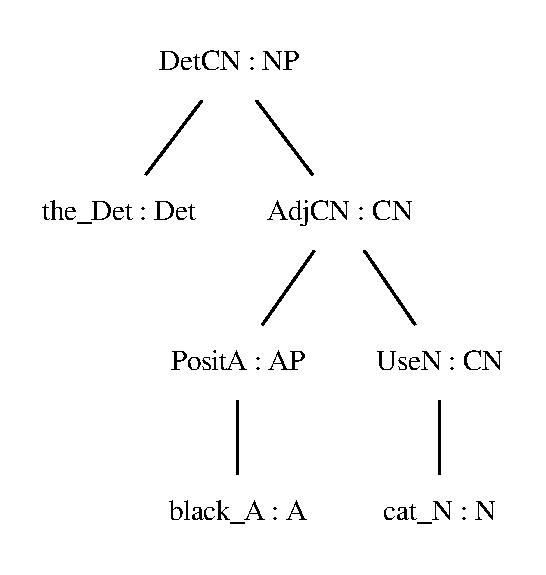
\includegraphics[scale=0.75]{thesis/figure/black_cats/the_black_cat_NP_gf.eps}}
    \caption{The four available trees on the word ``cat'' after the third iteration \emph{before} pruning. Trees (a) and (c) are both subtrees of the final tree (d), while tree (b) is not a subtree of (d), because it connects ``the'' directly to ``cat'' ignoring the adjective ``black''}\label{fig:cat iter 3}
\end{figure}


and like before, we get multiple trees of the same category, this time of type $NP$, once again allowing us to prune the less covering tree
\begin{lstlisting}
    DetCN the_Det (UseN cat_N) : NP
\end{lstlisting}

After this no more functions can be applied at the ``cat'' node, giving us a final set of cat trees (\autoref{fig:cat iter 3 pruned})
\begin{lstlisting}
    cat_N : N
    ModCN (PositA black_A) (UseN cat_N) : CN
    DetCN the_Det (ModCN (PositA black_A) (UseN cat_N)) : NP
\end{lstlisting}

\begin{figure}
    \centering
    \subcaptionbox{Cat : N\label{ci3p:cat_N}}
        {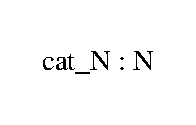
\includegraphics[scale=0.75]{thesis/figure/black_cats/cat_N_gf.eps}}
    \subcaptionbox{Black cat : CN\label{ci3p:black_cat_CN}}
        {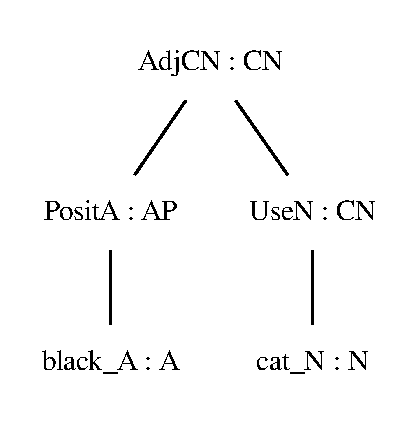
\includegraphics[scale=0.75]{thesis/figure/black_cats/black_cat_CN_gf.eps}}
    \subcaptionbox{The black cat : NP\label{ci3p:the_black_cat_NP}}
        {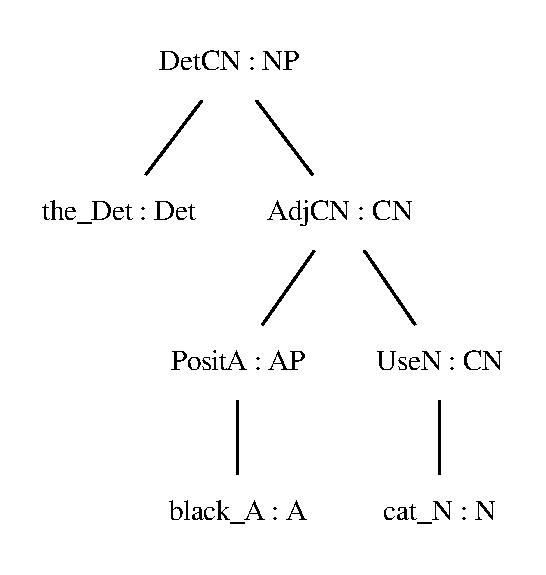
\includegraphics[scale=0.75]{thesis/figure/black_cats/the_black_cat_NP_gf.eps}}
    \caption{The three available trees on the word ``cat'' after the third iteration \emph{after} pruning. Trees (a) and (b) are both subtrees of the final tree (c)}\label{fig:cat iter 3 pruned}
\end{figure}

Now finally we have a complete tree which contains all of the words of the phrase, so we will choose the tree in \autoref{ci3p:the_black_cat_NP} as the final tree. 

In the end, the data structure used in the calculation will look like in \autoref{fig:final nested tree}, with the UD-structure outside which we traverse in order to find which parts can be connected and in each node of this tree a list of the GF trees that are possible to construct using the words in the local UD-subtree, while conforming to the UD-labels. In this case, the word ``the'' one GF-tree, the word ``black'' has two possible trees and the word ``cat'', which also contains (?) the words ``the'' and ``black'' has four possible trees. 

\begin{figure}
    \centering
    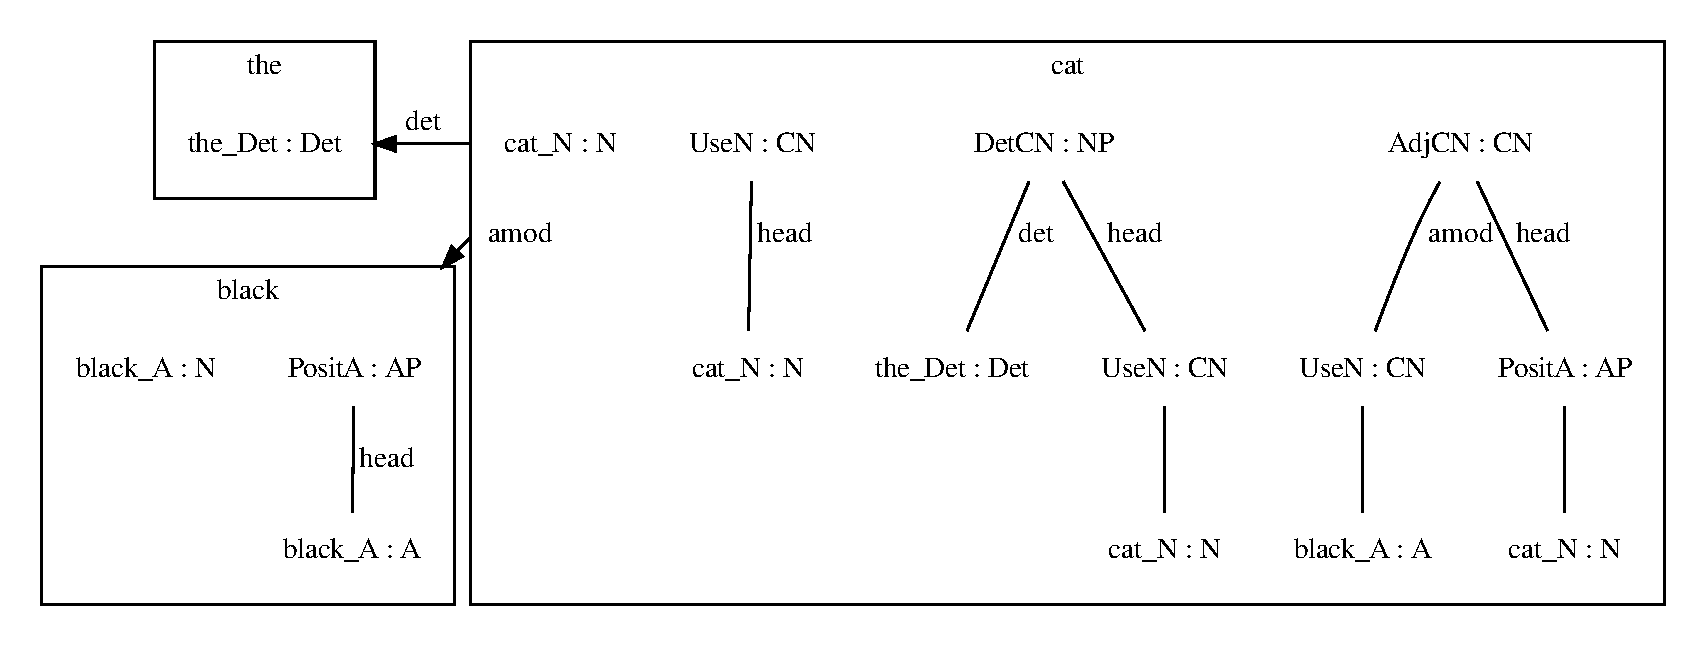
\includegraphics[width=0.7\textwidth]{figure/black_cats/the_black_cat_graph}
    \caption{An overview of the nested tree, with the UD structure outside and a list of GF-trees at each node}\label{fig:final nested tree}
\end{figure}


\begin{figure}
    \centering
    %% the black cat
    \setlength{\unitlength}{0.2mm}
    \begin{dependency}
        % TODO: Maybe don't center each line here
        \begin{deptext}[column sep=0.4cm]
              the\_Det : Det \& black\_A : A \& cat\_N : N \\
            \& PositA black\_A : AP \& UseN cat\_N : CN \\
            \& \& DetCN the\_Det (UseN cat\_N) : NP \\
            \& \& AdjCN (PositA black\_A) (UseN cat\_N) : CN \\
        \end{deptext}
        \depedge{3}{1}{det}
        \depedge{3}{2}{amod}
        \deproot{3}{root}
    \end{dependency} \\
    \caption{An overview of the nested tree, with the UD structure outside and a list of GF-trees at each node}
    \label{fig:final_nested_compact}
\end{figure}


\section{Differences between versions}

In the version 2 algorithm, in each iteration for a node in the UD tree (which corresponds to a word), after we have applied all possible functions and want to check if that unlocked new possible function applications, we check with \emph{all} the available trees in that node against each available function. This means that all the trees that were possible to construct in the previous iteration are still possible to construct, so we will construct them again and will need to remove the duplicates afterwards.


